\documentclass{article}

\usepackage{amsmath}
\usepackage{amssymb}

\usepackage{amsthm}
\theoremstyle{plain}
  \newtheorem{theorem}{Theorem}
  \newtheorem{lemma}[theorem]{Lemma}
  \newtheorem{proposition}[theorem]{Proposition}
  \newtheorem{conjecture}[theorem]{Conjecture}
  \newtheorem{corollary}[theorem]{Corollary}
\theoremstyle{definition}
  \newtheorem{definition}[theorem]{Definition}
  \newtheorem{remark}[theorem]{Remark}
  \newtheorem{example}[theorem]{Example}
  \newtheorem{procedure}[theorem]{Procedure}
  \newtheorem{assumption}[theorem]{Assumption}
\numberwithin{theorem}{section}

\usepackage{color}
\usepackage{graphicx}
\usepackage{geometry}

% bibliography
\usepackage[%
  backend=bibtex,bibencoding=ascii,
  style=numeric-comp,
  giveninits=true, uniquename=init, %abbreviate first names
  natbib=true,
  url=true,
  doi=true,
  isbn=false,
  backref=false,
  maxnames=99,
  ]{biblatex}
\addbibresource{references.bib}

\newcommand{\order}{{\mathcal O}}
\newcommand{\todo}[1]{{\Large{\color{red}{#1}}}}


\title{Notes on analysis of the KdVH equation}

\begin{document}

\maketitle

The KdVH system is

\begin{subequations} \label{kdvh}
\begin{align}
    u_t + uu_x + w_x & = 0 \\
    \tau_1 v_t - v_x & = -w \\
    \tau_2 w_t + u_x & = v.
\end{align}
\end{subequations}
We will often take $\tau_1 = \tau_2 = \tau$.

\section{Scaling symmetry}
The system \eqref{kdvh} is invariant under the following
transformation, for any $\epsilon>0$:
\begin{subequations}
\label{eq:scaling}
\begin{align}
    \tau_1 & \to \epsilon^2 \tau_1 & \tau_2 & \to \epsilon^4 \tau_2 \\
    x & \to \epsilon x & t & \to \epsilon^3 t \\
    u & \to \epsilon^{-2} u & v & \to \epsilon^{-3} v \\
    w & \to \epsilon^{-4} w.
\end{align}
\end{subequations}


\section{Asymptotic expansion}
We assume there exist power series for $u, v, w$ in terms of $\tau$:
\begin{align}
    u & = u^0 + \tau u^1 + \tau^2 u^2 + \cdots
    v & = v^0 + \tau v^1 + \tau^2 v^2 + \cdots
    w & = w^0 + \tau w^1 + \tau^2 w^2 + \cdots
\end{align}
Inserting these into \eqref{kdvh} and collecting terms we obtain the following.

$\order(\tau^0)$:
\begin{subequations}
\begin{align}
    v^0 & = u^0_x \\
    w^0 & = v^0_x \\
    u^0 + u^0 u^0_x + w^0_x & = 0.
\end{align}
\end{subequations}

(fill in the rest of the derivation here)

Finally we obtain (KdVH1)
\begin{align} \label{kdvh1}
    u_t + u u_x + u_{xxx} - \tau\left(u-u_{xx}  \right)_{xxt} - \tau^2\left(2u-u_{xx}\right)_{xxxtt} & = \order(\tau^3).
\end{align}

It would be straightforward to obtain additional terms in this equation if we think that would
be useful.

\section{Characteristic form}
For the homogeneous hyperbolic part of KdVH, the eigenvalues of the flux Jacobian are
\begin{align}
    \lambda_0 & = -1/\tau \\
    \lambda_\pm & = \frac{u}{2} \pm \frac{\sqrt{u^2 +4/\tau}}{2}.
\end{align}
The Riemann invariants are given by $v$ and
\begin{align}
\nu_\pm & = w + \frac{u}{2} \lambda_\pm \pm \frac{\log(\lambda_+)}{\tau}.
\end{align}
Note that the system has two genuinely nonlinear fields and one linearly
degenerate field.

In terms of these quantities, the full system \eqref{kdvh} can be written
\begin{subequations}
\begin{align}
    v_t - \frac{1}{\tau} v_x & = -\frac{1}{\tau} w \\
    (\nu_\pm)_t + \lambda_\pm (\nu_\pm)_x & = \frac{1}{\tau} v.
\end{align}
\end{subequations}
It may be useful to express $w$ in terms of the Riemann invariants
in order to better understand this system.



\section{Regularity results}

Following Dafermos \cite[Section~5.2]{dafermos2010hyperbolic}, we write the KdVH system \eqref{kdvh} as
\begin{equation}
\begin{aligned}
    \partial_t U + \partial_x G(U) + P(U) &= 0, && x \in \mathbb{R}, t > 0, \\
    U(x, 0) &= U_0(x), && x \in \mathbb{R},
\end{aligned}
\end{equation}
where $U = (u, v, w)^T$, the flux function is
\begin{equation}
    G(U) = \left( \frac{1}{2} u^2 + w, -\tau_1^{-1} v, \tau_2^{-1} u \right)^T,
\end{equation}
and the source term is
\begin{equation}
    P(U) = \left( 0, \tau_1^{-1} w, -\tau_2^{-1} v \right)^T.
\end{equation}
In their notation, $\overline{U} = 0$ is indeed a constant equilibrium.
Furthermore,
\begin{equation}
    \eta(U) = \frac{1}{2} u^2 + \frac{\tau_1}{2} v^2 + \frac{\tau_2}{2} w^2
\end{equation}
is a uniformly convex entropy satisfying
\begin{equation}
    \partial_t \eta(U) + \partial_x Q(U) + \underbrace{\eta'(U) P(U)}_{= 0} = 0,
\end{equation}
where
\begin{equation}
    Q(U) = \frac{1}{6} u^3 + u w - \frac{1}{2} v^2
\end{equation}
is the associated entropy flux. Note that
\begin{equation}
    P'(U) = \begin{pmatrix}
        0 & 0 & 0 \\
        0 & 0 & \tau_1^{-1} \\
        0 & -\tau_2^{-1} & 0
    \end{pmatrix}.
\end{equation}
Thus, the source term $P$ is not strongly dissipative in the sense of \cite[Section~5.2, p.~109]{dafermos2010hyperbolic}.
However, the assumption \cite[(5.2.12)]{dafermos2010hyperbolic} is satisfied for $\tau_1 \ne 0 \ne \tau_2$, i.e.,
\begin{equation}
    P'(\overline{U}) R_i(\overline{U}) \ne 0, \qquad i \in \{1, 2, 3\},
\end{equation}
since the eigenvectors $R_i$ of the flux Jacobian $G'(U)$ are \cite{besse2022perfectly}
\begin{equation}
    \begin{pmatrix}
        0 \\ 1 \\ 0
    \end{pmatrix},
    \quad
    \begin{pmatrix}
        *_+ \\ 0 \\ 1
    \end{pmatrix},
    \quad
    \begin{pmatrix}
        *_- \\ 0 \\ 1
    \end{pmatrix}.
\end{equation}
Thus, \cite[Theorem~5.2.1]{dafermos2010hyperbolic} applies, and we obtain the following result.
\begin{theorem}
\label{thm:small_data}
    Let
    $\tau_1, \tau_2 > 0$,
    $\ell > 1$,
    $U_0 \in L^2(\mathbb{R})$,
    $\nabla U_0 \in H^\ell$, and
    $\|\nabla U_0\|_{H^\ell}$ be sufficiently small.
    Then, there is a unique global classical solution $U$ of the Cauchy problem for the KdVH system \eqref{kdvh}.
\end{theorem}

By using the scaling symmetry \eqref{eq:scaling}, we can also obtain a similar result for large initial data, but small $\tau_1, \tau_2$.
\begin{theorem}
\label{thm:small_tau}
    Let
    $U_0 \in L^2(\mathbb{R})$ and
    $\nabla U_0 \in H^1$.
    Then, there are $\tau_1, \tau_2 > 0$ sufficiently small such that
    there is a unique global classical solution $U$ of the Cauchy problem for the KdVH system \eqref{kdvh}.
\end{theorem}
\begin{proof}
    Applying the scaling \eqref{eq:scaling} yields
    \begin{equation}
        \| \nabla u_0 \|_{L^2} \mapsto \epsilon^{3/2} \| \nabla u_0 \|_{L^2}, \qquad
        | \nabla u_0 |_{H^1} \mapsto \epsilon^{1/2} | \nabla u_0 |_{H^1}.
    \end{equation}
    The other components $v_0, w_0$ behave in the same way if they are initialized with well-prepared initial data, i.e., $v_0 = \partial_x u_0$ and $w_0 = \partial_{xx} u_0$.
    Thus, we can choose $\epsilon$ (and consequently $\tau_1$ and $\tau_2$) sufficiently small such that $\|\nabla U_0\|_{H^1}$ is sufficiently small after the scaling to apply Theorem~\ref{thm:small_data}.
\end{proof}

This sheds more light on how the convergence of (possibly discontinuous, weak entropy) solutions of KdVH to smooth solutions of KdV as $\tau_1, \tau_2 \to 0$ \cite[Theorem~3.2]{giesselmann2025convergence} happens.
Indeed, for given initial data, there are critical thresholds for $\tau_1, \tau_2$ below which there are only classical solutions on KdVH.

Using the scaling symmetry \eqref{eq:scaling} the other way round, we notice that KdVH may have discontinuous solutions for any $\tau_1, \tau_2 > 0$ as long as the initial data are sufficiently big (in the sense of $\| U_0 \|_{H^\ell}$ not being small).

\todo{TODO: Check well-posedness results for KdV}

\todo{TODO: Can we reverse-engineer relative energy convergence results to show well-posedness of KdV using this?}


\section{Some numerical results}

The results currently included here are computed using a 1st-order HLL solver.  It should be
kept in mind that this is quite dissipative so longer-time solutions will not be accurate.

For all of these solutions the initial condition is
\begin{align}
    u(x,t=0) = 2 \exp(-x^2/50).
\end{align}

In Figure \ref{fig:convergence}, we observe visual convergence to the KdV solution as
$\tau$ is decreased.

\begin{figure}
\centering
    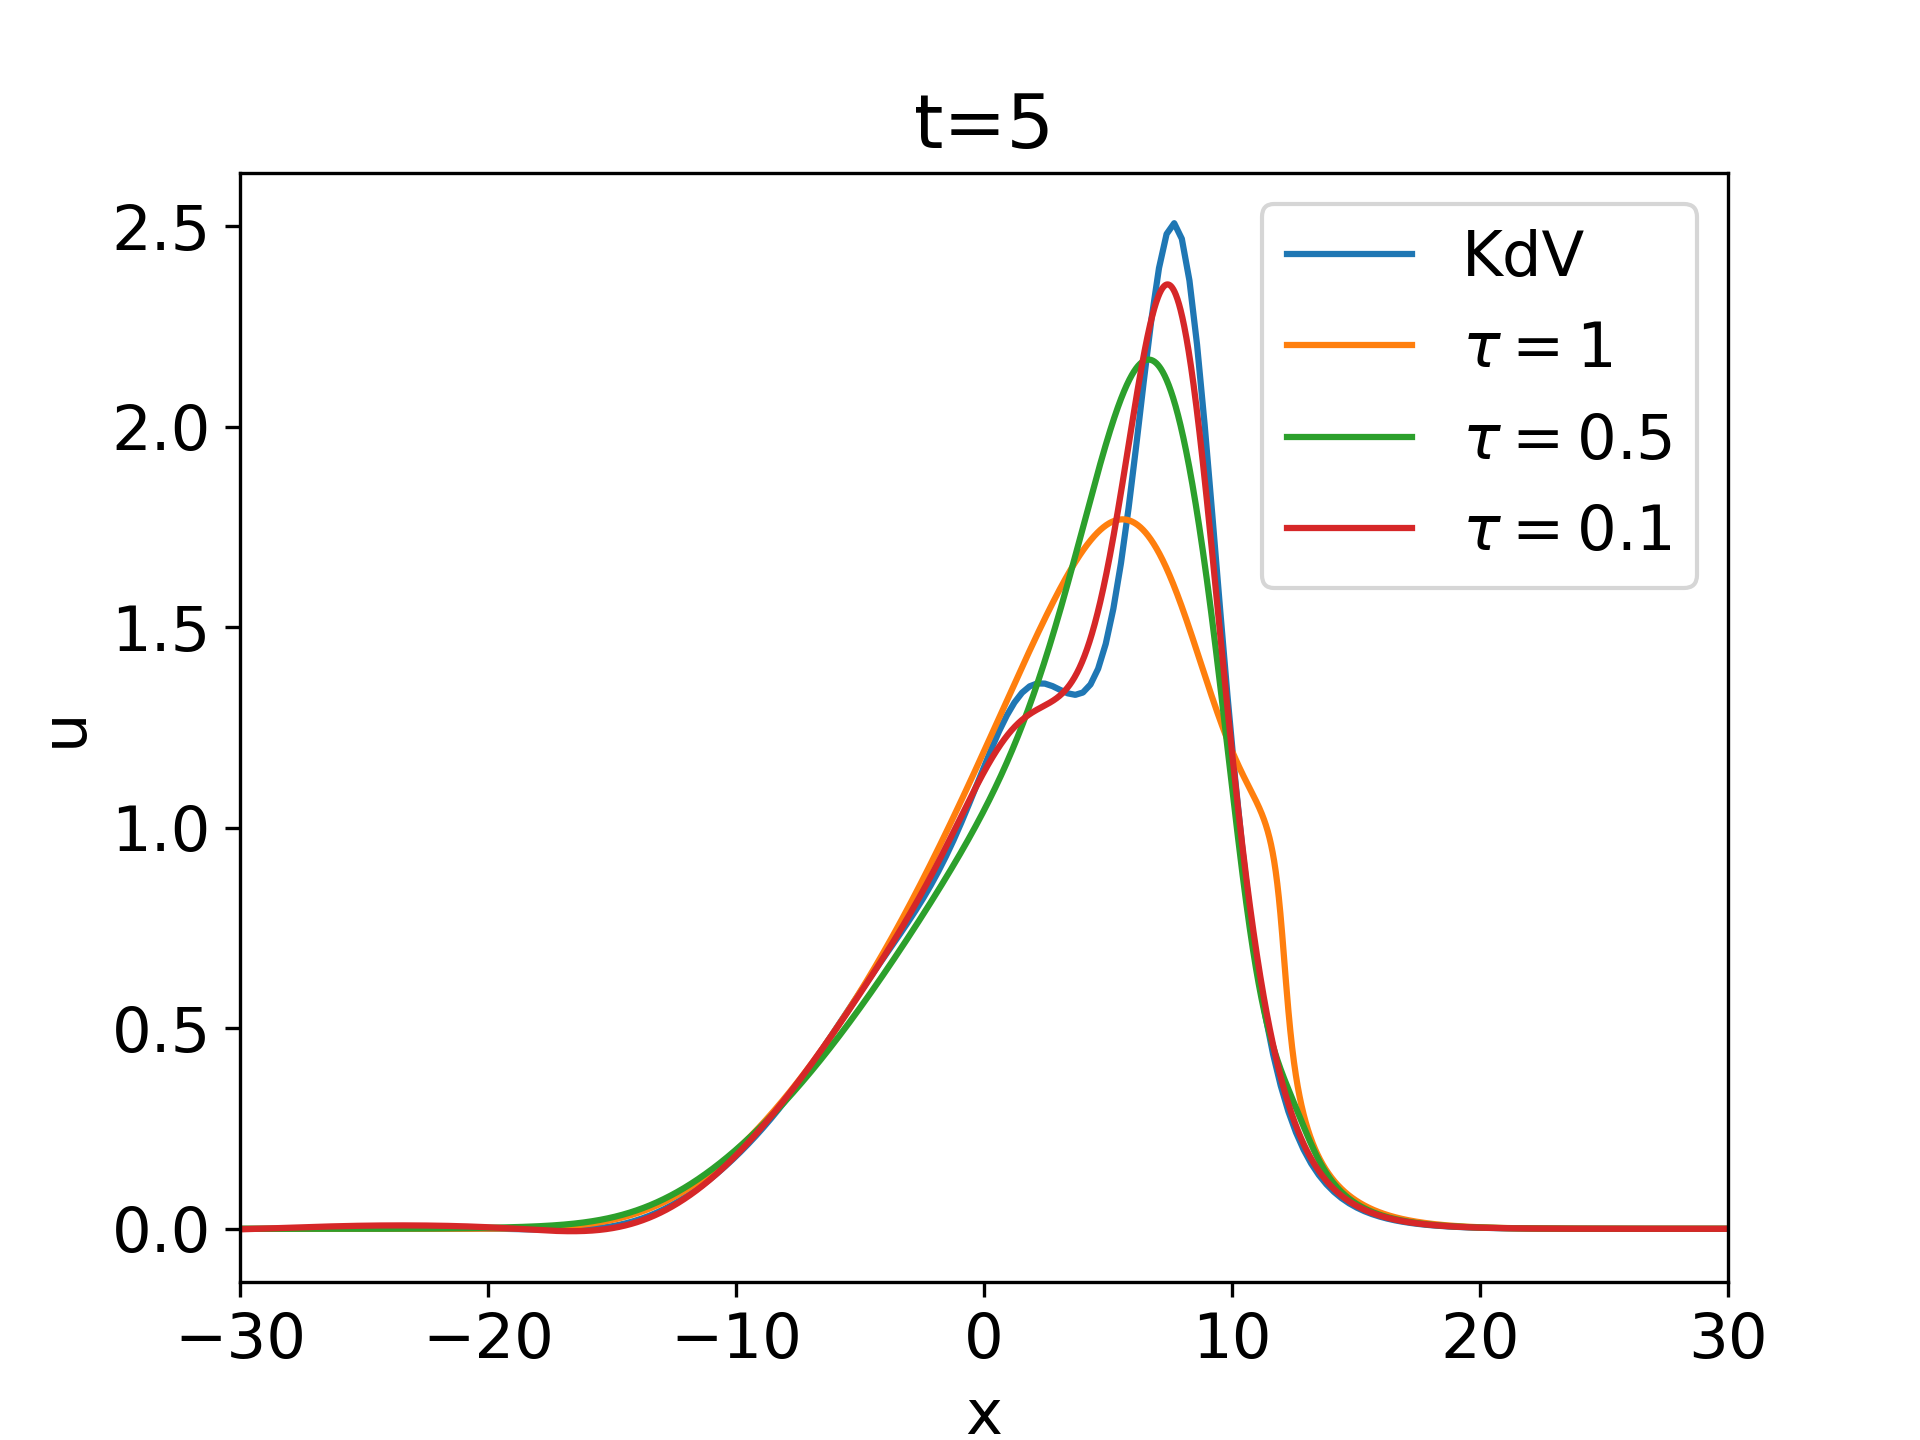
\includegraphics[width=4in]{figures/Convergence.png}
    \caption{Convergence of KdVH solutions to KdV.\label{fig:convergence}}
\end{figure}

In Figure \ref{fig:shocks}, we observe the clear appearance of shocks for $\tau=1$, while
the solution for $\tau=1/10$ is clearly devoid of shocks.

\begin{figure}
\centering
    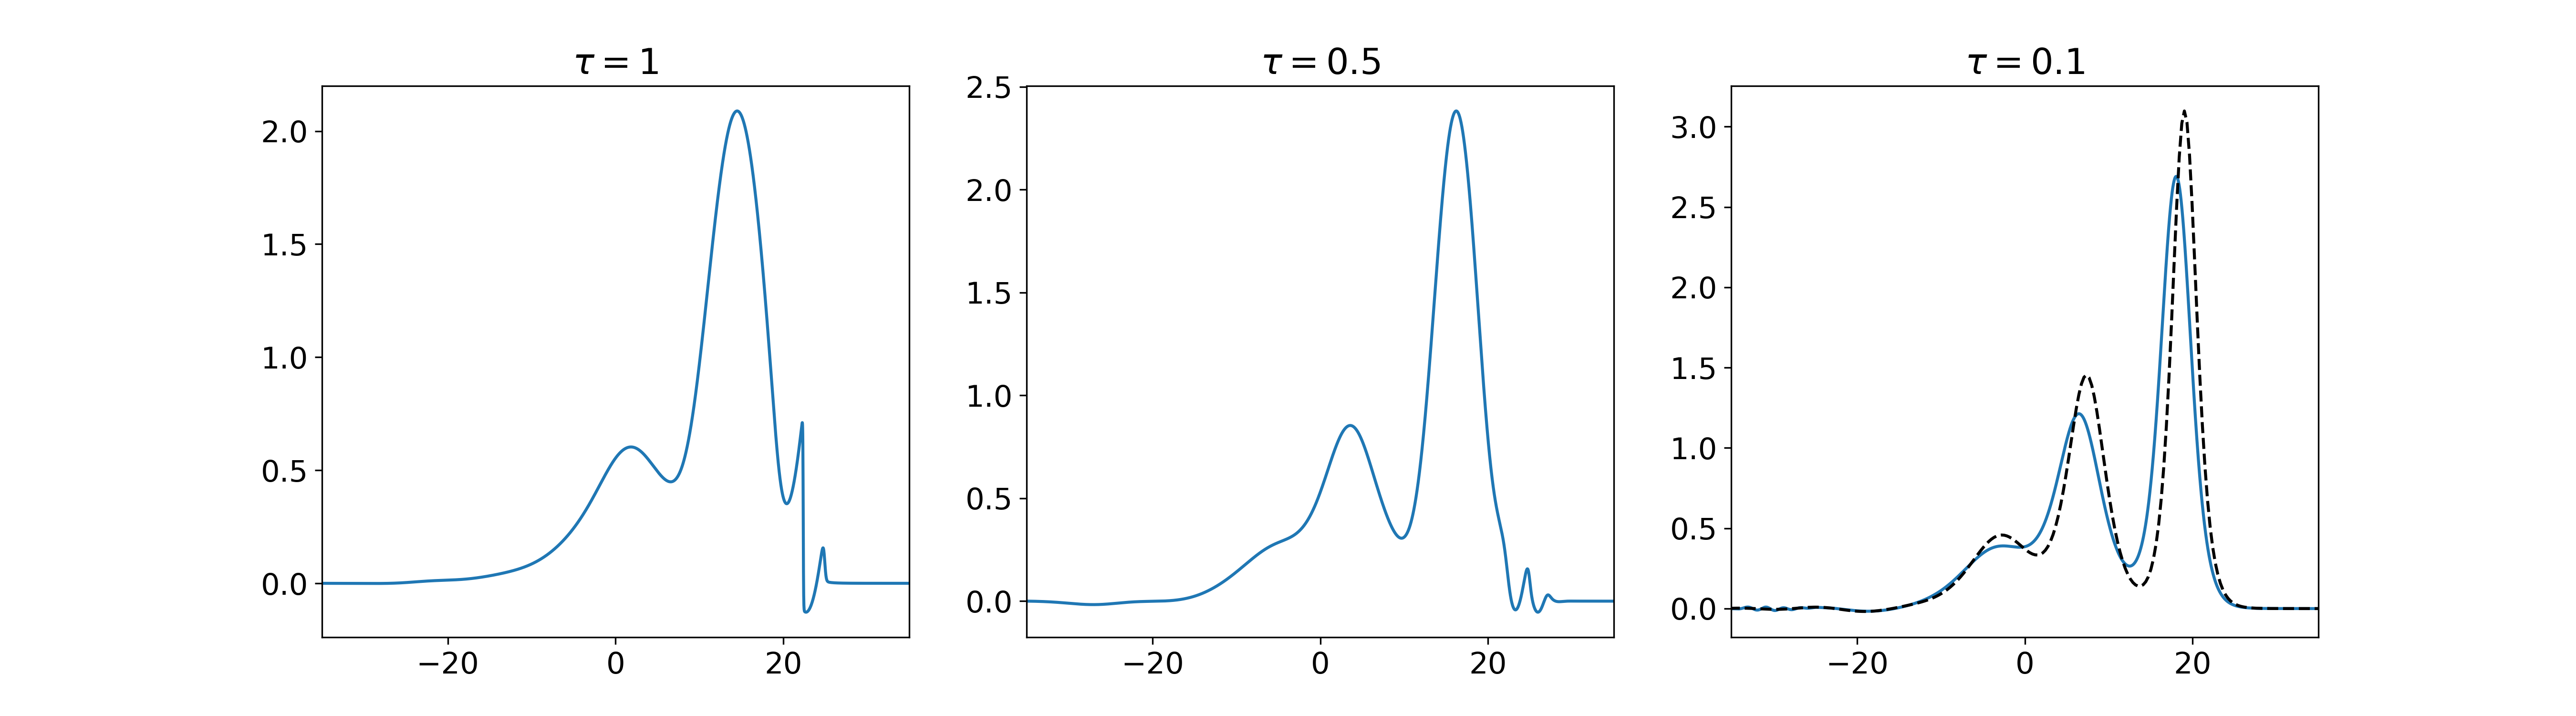
\includegraphics[width=6in]{figures/KdVH_solutions.png}
    \caption{Comparison of solutions at $t=16$.  In the last plot, the KdV solution is included (dashed black line)
    for comparison.\label{fig:shocks}}
\end{figure}


\todo{TODO}



\section{Summary and discussion}

\todo{TODO}



\appendix

\section*{Acknowledgments}

\todo{TODO: funding}
% \input{funding}


\printbibliography

\end{document}

